%template1.tex
%The following LaTeX source file represents the simplest kind of slide presentation; no overlays, no included graphics. Substitute your favorite style for ``pascal''. To create the PDF file template1.pdf, (1) be sure to use the prosper class, then (2) execute the command latex template1.tex, and (3) the command dvipdf template1.dvi.

%%%%%%%%%%%%%%%%%%%%%%%%%%%%%%% template1.tex %%%%%%%%%%%%%%%%%%%%%%%%%%%%%%%%%%%
\documentclass[a4paper,blends,pdf,colorBG,slideColor]{prosper}
% definitions for slides for CSC544
% Lutz Hamel, (c) 2007

\hypersetup{pdfpagemode=FullScreen}

\usepackage{times}
\usepackage{latexsym}
\usepackage{alltt}
\usepackage{booktabs}
\usepackage{amsmath}
\usepackage{amsopn}
\usepackage{amsfonts}
\usepackage{amssymb}
%\usepackage[usenames]{color}

\def\sign{\qopname\relax{no}{sign}}
\def\argmax{\qopname\relax{no}{argmax}}
\def\argmin{\qopname\relax{no}{argmin}}

\newcommand{\grad}{\ensuremath{\nabla}} 
\newcommand{\loss}{\ensuremath{{\cal L}}}
\newcommand{\err}{\mbox{err}}
\newcommand{\mse}{\mbox{mse}}
\newcommand{\acc}{\mbox{acc}}
\newcommand{\Integer}{\ensuremath{\mathbb{N}}}
\newcommand{\size}[1]{{|{#1}|}}
\newcommand{\Rnspace}[1]{\ensuremath{\mathbb{R}^{#1}}}
\newcommand{\Real}{\ensuremath{\mathbb{R}}}
\newcommand{\mytt}[1]{{\small\tt{#1}}}
\newcommand{\textemph}[1]{{\em #1}}
\newcommand{\suchthat}{\mid}
\newcommand{\orbar}{\;|\;}
\newcommand{\bs}[1]{\begin{slide}{#1}\ptsize{8}}
\newcommand{\es}{\end{slide}}
\newcommand{\co}{\,\colon\;}
\newcommand{\pair}[2]{\ensuremath{( {#1}, {#2} )}}
\newcommand{\model}[1]{\hat{#1}}
\newcommand{\ul}[1]{{\bf\em #1}}
\newcommand{\ol}{\overline}
\newcommand{\definition}[1]{{\bf Definition: }{\em #1}}
\newcommand{\example}[1]{{\bf Example: }{#1}}
\newcommand{\abs}[1]{|{#1}|}
\newcommand{\mytab}{\makebox[.1in]{}}

\newcommand{\fdef}[1]{
\begin{center}
\fbox{
\begin{minipage}{3.5in}
{\bf Definition:}
{#1}
\end{minipage}
}
\end{center}
}

\newcommand{\fframe}[1]{
\begin{center}
\fbox{
\begin{minipage}{3.5in}
{#1}
\end{minipage}
}
\end{center}
}

\newcommand{\nframe}[1]{
\begin{center}
\begin{minipage}{3.5in}
{#1}
\end{minipage}
\end{center}
}

\newenvironment{Rcode}
	{
		\scriptsize
		\begin{quote}
		\begin{alltt}
	}
	{
		\end{alltt}
		\end{quote}
	}




\begin{document}

\bs{Leave-One-Out}

{\bf Observations:} 
\begin{itemize}
\item The quality of the test error estimate $\err_Q$
in the hold-out method 
greatly depends on the random split of the data set $D$ into a training set and a
test set.  
\item A poorly executed split can adversely affect the model evaluation.

\item One way to mitigate the bias of the random split of $D$ is to perform the split-train-test cycle multiple times.
\end{itemize}
\es

\bs{Leave-One-Out}
%\small
In the leave-one-out method  we split the data set $D$ of size $l$
into $l$ partitions of size $1$ such that,
\begin{equation*}
D = Q_1\cup Q_2 \cup \ldots \cup Q_{l-1} \cup Q_{l},
\end{equation*}
and
\begin{equation*}
Q_i \cap Q_j = \emptyset,
\end{equation*}
where $Q_i = \{ (\ol{x}_i, y_i)\}$ and $Q_j = \{ (\ol{x}_j, y_j)\}$
for $i,j = 1,\ldots, l$ and $i \ne j$.

Each partition $Q_i$ is used systematically for testing exactly once whereas the
remaining  partitions are used for training.  
Let $P_i = D - Q_i$ be the training set with respect to the test partition $Q_i$ with $i = 1,\ldots, l$,
then we can compute the error for each test partition as
\begin{equation*}
\err_{Q_i}\left [\model{f}_{P_i}[k,\lambda,C]\right] = \loss\left (y_i,\model{f}_{P_i}[k,\lambda,C](\ol{x}_i)\right ),
\end{equation*}
where $\model{f}_{P_i}[k,\lambda,C]$
is the model trained on data set $P_i$ with parameters $k$, $\lambda$, and $C$.

The test error $\err_{Q_i}$ is computed as the loss over the single element in the test partition $Q_i$.

\es

\bs{Leave-One-Out}

The {\em leave-one-out error} (LOOE) is the average error over all partitions,
\begin{equation*}
\text{LOOE}_D\left [k,\lambda,C \right ] 
	= \frac{1}{l} \sum_{i=1}^l \err_{Q_i}\left [\model{f}_{P_i}[k,\lambda,C]\right].
\end{equation*}

{\bf Observation:} The leave-one-out error
is an error estimate only in terms of the {\em model parameters}.

We can compute the set of parameters that minimizes the leave-one-out error over all partitions as,
\begin{equation*}
(k^*,\lambda^*,C^*) = \argmin_{k,\lambda,C} \text{LOOE}_{\color{red}D}\left [k,\lambda,C \right ] ,
\end{equation*}
and this parameter set gives rise to the optimal model
\begin{equation*}
\model{f}_{\color{red}D}[k^*,\lambda^*,C^*].
\end{equation*}

\es

\bs{Leave-One-Out}
\vspace{.2in}
{\bf Observation:} For a data set $D$ of length $l$ we have to build $l$ models for each parameter set
evaluation.  
This implies that for most real-world data sets whose lengths is in the thousands and perhaps millions of
observations this approach becomes unfeasible.
\es


\bs{$N$-Fold Cross-Validation}
\small
A good compromise between the potential bias of the hold-out method and the computational
complexity of the leave-one-out method is {\em $N$-fold cross-validation}.  

Here we split the data set $D$ into $N$ partitions or \textemph{folds} with $N \ll l$ such that
\begin{equation*}
D = Q_1\cup Q_2 \cup \ldots \cup Q_{N-1} \cup Q_{N},
\end{equation*}
and
\begin{equation*}
Q_i \cap Q_j = \emptyset,
\end{equation*}
with $\size{Q_i} = \size{Q_j} = l/N$ for $i,j = 1,\ldots, N$ and $i \ne j$.

We will use each  fold for testing exactly once and the remaining  folds
are used to train the models.   Let $Q_i$  be a
fold of the dataset $D$,
 then we can construct our corresponding training set $P_i$
as
\begin{equation*}
P_i = D - Q_i,
\end{equation*}
with $i = 1,\ldots,N$.
We can compute the error of some fold $Q_i$ as
\begin{equation*}
 \err_{Q_i}\left [\model{f}_{P_i}[k,\lambda,C]\right] = \frac{1}{\size{Q_i}}\sum_{(\ol{x}_j, y_j) \in Q_i}\loss\left (y_j,\model{f}_{P_i}[k,\lambda,C](\ol{x}_j)\right ),
\end{equation*}
where $\model{f}_{P_i}[k,\lambda,C]$
is the model trained on dataset $P_i$ with parameters $k$, $\lambda$, and $C$.

\es

\bs{$N$-Fold Cross-Validation}

We compute the {\em cross-validated error} (CVE) of the parameter set $k$, $\lambda$, and
$C$ as the average over the individual fold errors,
\begin{equation*}
\text{CVE}_D\left [k,\lambda,C \right ] 
	= \frac{1}{N} \sum_{i=1}^N \err_{Q_i}\left [\model{f}_{P_i}[k,\lambda,C]\right].
\end{equation*}

And we find the optimal parameter set by minimizing the
cross-validated error,
\begin{equation*}
(k^*,\lambda^*,C^*) = \argmin_{k,\lambda,C} \text{CVE}_D\left [k,\lambda,C \right ] .
\end{equation*}
The optimal model $\model{f}_D[k^*,\lambda^*,C^*]$ can then be constructed using 
the full data set $D$.

\es

\bs{$N$-Fold Cross-Validation}
\vspace{.2in}
\scriptsize
\begin{Rcode}
> svm.model <- svm(Diagnosis ~ ., 
                   data=wdbc.df, 
                   type="C-classification",
                   kernel="polynomial", 
                   degree=3, 
                   cost=1000,
                   {\color{red}cross=10})
> summary(svm.model)

{\color{red}10-fold cross-validation on training data:}

Total Accuracy: 94.55185 
Single Accuracies:
 91.07143 94.73684 98.24561 96.49123 100 
 87.7193 94.73684 94.73684 94.73684 92.98246 
\end{Rcode}
\es

\bs{$N$-Fold Cross-Validation}
\scriptsize
   \begin{tabular*}{\textwidth}{@{\extracolsep{\fill}} llrrr}
      \toprule
       ID & Kernel & Cost Constant & Training Error & Cross-Validated Error\\
      \midrule
     1& Linear & 0.01&   $2.46\%$& $3.51\%$ \\
     2& Linear & 0.10&    $1.41\%$ & $2.46\%$ \\
      3&Linear & 1.00 &   $1.23\%$ & $2.81\%$\\
      4&Linear & 10.00 &   $0.88\%$ & $3.34\%$\\
      5&Linear & 100.00 &   $0.35\%$ & $3.34\%$\\
      6&Linear & 1000.00 &   $0.35\%$ & $3.87\%$\\
      7&Polynomial, $\text{degree}=3$ & 10.00 & $2.81\%$ & $4.39\%$\\
      8&Polynomial, $\text{degree}=3$ & 100.00 & $0.53\%$ & $3.34\%$\\
      9&Polynomial, $\text{degree}=3$ & 1000.00 & $0.00\%$ & $5.45\%$\\
      \bottomrule
   \end{tabular*}

\begin{center}
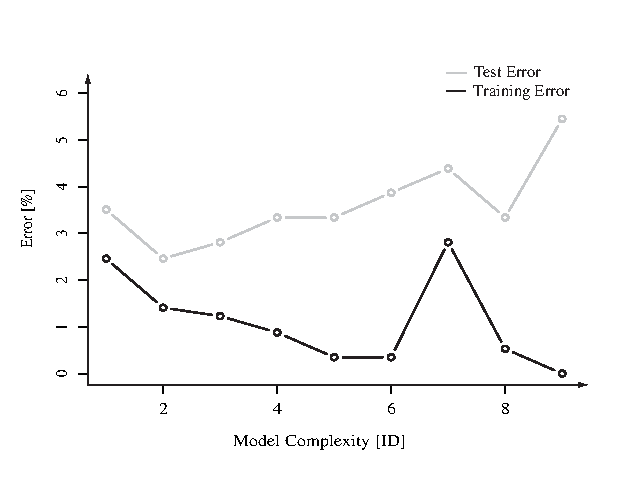
\includegraphics[height=30mm]{figures/fig09-05.eps}
\end{center}
\es
\end{document}
%%%%%%%%%%%%%%%%%%%%%%%%%%% end of template1.tex %%%%%%%%%%%%%%%%%%%%%%%%%%%%%%%%

